% This is samplepaper.tex, a sample chapter demonstrating the
% LLNCS macro package for Springer Computer Science proceedings;
% Version 2.20 of 2017/10/04
%
\documentclass[runningheads]{llncs}
%
\usepackage{graphicx}
\usepackage{amsmath}
\usepackage{amssymb}
\usepackage{helvet,times,courier}
\usepackage{listings}
\usepackage[inline]{enumitem}
\lstset{numberbychapter=false,numbers=left,numberblanklines=false,basicstyle=\footnotesize\ttfamily,xleftmargin=5ex}
% Used for displaying a sample figure. If possible, figure files should
% be included in EPS format.
%
% If you use the hyperref package, please uncomment the following line
% to display URLs in blue roman font according to Springer's eBook style:
% \renewcommand\UrlFont{\color{blue}\rmfamily}

\begin{document}
%
\title{A decomposition Approach for solving the JSP using multi-shot ASP\thanks{Supported by organization x.}}
%
%\titlerunning{Abbreviated paper title}
% If the paper title is too long for the running head, you can set
% an abbreviated paper title here
%
\author{Mohammed M. S. El-Kholany\inst{1}\orcidID{0000-0002-1088-2081} \and
Martin Gebser\inst{1,2}\orcidID{0000-0002-8010-4752} \and
Konstantin Schekotihin\inst{1}\orcidID{0000-0002-0286-0958}}
%
\authorrunning{M. El-Kholany et al.}
% First names are abbreviated in the running head.
% If there are more than two authors, 'et al.' is used.
%
\institute{Alpen-Adria-Universität Klagenfurt, Klagenfurt, Austria 
\email{\{mohammed.el-kholany, martin.gebser and konstantin.schekotihin\}@aau.at}\\
%\url{http://www.springer.com/gp/computer-science/lncs} \and
Technische Universität Graz, Graz, Austria\\
\email{mgebser@ist.tugraz.at}}
%
\maketitle              % typeset the header of the contribution
%
\begin{abstract}
The abstract should briefly summarize the contents of the paper in
150--250 words.

\keywords{Job-shop Scheduling Problem  \and Answer Set Programming \and Decomposition.}
\end{abstract}
%
%
%
\section{Introduction}
In today's competitive markets, manufacturers have to respond quickly to orders and meet shipping dates committed to the customers. This requires the ability to schedule production activities to use the available scarce resources efficiently. Effective scheduling techniques are essential in complex manufacturing systems such as semiconductor manufacturing. In general, scheduling operations is one of the most critical issues in the planning and managing of the manufacturing processes\cite{uzsoy2000performance}. 

One of the most challenging scheduling problems is the Jop-shop Scheduling Problem (JSP). A set of jobs needs to be processed on a set of machines while optimizing a performance indicator, minimizing makespan, the time needed to complete all the jobs, or tardiness, i.e., the summation of the delays in executing all jobs according to their deadlines. Each job has a set of consecutive operations; each operation requires exactly one machine; machines are continuously available and can process only one operation at a time. The main purpose is to determine the sequence of the operations on each machine to optimize a performance indicator. The JSP is an NP-complete combinatorial optimization problem where obtaining the optimal solution is challenging regardless of the problem scale\cite{garey1976complexity,lenstra1977complexity,liu2008prediction}. For instance, benchmark (FT10) consists of $10$ jobs and $10$ machines took researchers roughly $20$ years to find the optimal solution\cite{adams1988shifting,zhang2010hybrid}.

In reality, the number of operations is reaching thousands of operations. Therefore, the exact methods Answer Set Programming (ASP), Constraint Programming and Branch and Bound cannot find the optimal solutions in a reasonable time\cite{daneshamooz2021mathematical,shi2021solving,francescutto2021solving}. Since the performance of the exact methods will be hardly satisfactory, several studies have presented one of the most effective methods for solving the JSP, which is decomposition \cite{zhang2010hybrid}. The decomposition aims to split the problem into a series of subproblems based on a particular decomposition policy and then solve each part separately and obtain the final solution by integrating all of these solutions. Several strategies have been proposed to decompose the JSP, and each varies according to the problem features. More specifically, there is no evidence that one of the introduced strategies is the best for solving all JSP(s) \cite{ovacik2012decomposition}. 

In this study, we aim to introduce a new decomposition strategy for solving the JSP. Our study proposes a new policy to efficiently divide the problem into subproblems, aiming to reach a near-optimal solution. Then each part is solved using an ASP scheduler-based, and the solutions are integrated to obtain the solution of the whole problem. We develop and implement our model using ASP, which is considered as one of the most popular paradigms for knowledge representation and reasoning, especially in combinatorial optimization problems \cite{abseher2016shift}. 

The paper is organized as follows. The following section shows the most related work and which decomposition techniques have been introduced in the past, followed by the problem formulation section illustrates the problem in detail. Section $4$ presents our proposed model, which shows the decomposition techniques we used and describes one in more detail. In addition, we present the schedule model using Answer Set Programming. Our model is tested by performing extensive experiments on a set of benchmark instances in Section $5$. Section $6$ summarizes this work and provides some ideas to extend the current work.

\section{Literature Review}
This section will review some of the work that has applied the decomposition approach for solving scheduling problems. As mentioned in the previous section, no particular decomposition method has proved its efficiency in solving all scheduling problems. However, many articles have introduced efficient decomposition methods for solving particular scheduling problems with specific features. The decomposition idea for solving JSP has been initially suggested by introducing a \textit{Shifting bottleneck} (SB) procedure which decomposes the problem into parts; each part contains only one machine \cite{adams1988shifting}. At each iteration, the bottleneck machine is determined from a set of unsequenced machines and then scheduled. Afterward, all the previously established sequences are locally reoptimized and iterate until all the machines have been sequenced. The idea of SB had been later improved by integrating an optimization algorithm for solving the one-machine problem with the delayed precedence constraints procedure \cite{balas1995one}.

Another study investigated the performance of a new decomposition procedure based on SB in the Job-shop and flow shop with different levels of bottleneck machines. The computational experiments showed that the proposed method obtained better solutions in a shorter time than for the problems in which the machine's workload is identical. Other different methods have been developed to decompose the JSP. For instance, a rolling horizon heuristic has been presented \cite{singer2001decomposition} to solve a large-scale job shop. The authors have decomposed the problem and solve each independently while minimizing the total weighted tardiness. They tested their model on a set of benchmark instances, and the results showed that the proposed model is superior to large instances. 

The rolling horizon procedure has been extended by constructing a prediction model to obtain the scheduling characteristics values, including the information of the bottleneck jobs. The obtained information aided in decomposing the problem efficiently. In addition, they have proposed a genetic algorithm to solve each sub-problem. In order to evaluate the performance of the proposed model, they performed numerical computational experiments that showed the effectiveness of the model \cite{liu2008prediction}. A decomposition-based hybrid optimization algorithm has been introduced for the JSP, where the total weighted tardiness is minimized. A Simulated Annealing is used to define subproblems iteratively and then is solved by a Genetic Algorithm. They have developed a fuzzy system that provides information about bottleneck jobs. This information is used to guide the process of subproblem-solving to promote the optimization efficiency \cite{zhang2010hybrid}. The numerical computational results showed that the proposed algorithm is effective for large-scale scheduling problems.

A decomposition method based on bottleneck machines has been presented for solving the JSP. The proposed model decomposes the problems into subproblems and then detects the multi-bottleneck machines using a critical path method. The information of the bottleneck machines has been employed to improve the solution quality by splitting the operations into bottleneck operations and non-bottleneck operations, where the bottleneck operations are scheduled by the Genetic Algorithm and the non-bottleneck operations are scheduled by dispatching rules \cite{zhai2014decomposition}.

From the literature, we can find that most of the related work focused on applying the decomposition approach while minimizing the total tardiness, and the number of work tackled large-scale instances to minimize the makespan is relatively low. This paper proposes different decomposition strategies for solving the JSP with larger instances using the ASP model while minimizing the makespan.

\section{Preliminaries}
\paragraph{Answer Set Programming (ASP)} is a declarative programming language for solving hard combinatorial optimization problems. ASP has become an established paradigm for knowledge representation and reasoning. ASP has proved its efficiency for solving the combinatorial optimization problem in different applications such as bioinformatics\cite{erdem2015generating,koponen2015optimizing}, databses\cite{caniupan2010consistency} and scheduling and industrial applications~\cite{dodaro2015allotment,dodaro2016combining,fabricius2020towards,dodaro2021operating}.

A logic program is a finite set of rules of the form 
\begin{equation}
	a_0 \gets a_1, \ldots, a_m, \sim a_{m+1}, \dots, \sim a_n
	\label{rule1}
\end{equation}
where $a_i$ is an atom for $0 \leq i \leq n$ and ``$\sim$''  is a default negation. If $n$ quals to $0$, then a rule \eqref{rule1} is a fact. If $a_0$ is omitted, the rule is an integrity constraint. An \emph{atom} is an expression of the form $p(t_1,\ldots,t_l)$, where $p$ is a predicate and $t_1,\ldots,t_l$ are \emph{terms}. Each term can be a variable or a constant. A \emph{literal} is either an atom or its negation. 
Given a rule $r$ of the form \eqref{rule1}, the set $H(r)=a_0$ denotes the \emph{head} atom and the set $B(r) = B^+(r) \cup B^-(r) = \{a_1,\dots,a_m\} \cup \{\sim a_{m+1}, \dots \sim a_n\}$ is the \emph{body} of $r$ where $B^+(r)$ and $B^+(r)$ represent the positive and negative body literals, respectively.
\paragraph{Multi-shot Solving:}
Multi-shot solving ASP allows solving logic programs dynamically in sequential order. This can be manipulated using APIs implementation via an imperative programming language. Such programming language is used to control the grounding and solving processes and allows the usage of external variables that could be set to $True$ or $False$ to control some logic rules. The main advantage of \emph{multi-shot} solving is to avoid the re-grounding and exploit conflicts learned over time.
%ASP is a paradigm that deals with continuously changing logic programs. In a single-shot approach, an ASP system takes a logic program, computes answer sets and exits. However, the idea of Multi-shot is to consider evolving grounding and solving processes. \emph{clingo} systems enhances the ASP declaritive language with control capacities. 
\paragraph{ASP Difference Logic:}
\emph{clingo}[DL] is an extension of the input language \emph{clingo} by theory atoms representing difference constraints \cite{gebser2016theory,janhunen2017clingo}. Difference constraints are defined by specific constraint atoms of the form $\text{\lstinline{&diff}}\{u-v\} \leq k$ where $u$ and $v$ are terms which are interpreted as integer variables and $k$ is an integer constant. \emph{clingo}[DL] provides the following extension of the normal form \eqref{rule1}: 
\begin{align*}
	\text{\lstinline{&diff}}\{u-v\} \leq k \gets a_1, \ldots, a_m, \sim a_{m+1}, \ldots, \sim a_n.
\end{align*}
 This rule shows that whenever the body is $True$ the inequality constraints must be satisfied.

\section{Problem Formulation}
The Job-shop Scheduling Problem (JSP) has been a complex and combinatorial optimization problem since the 1950s, and it was shown to be NP-hard. In the JSP, there are a set of jobs to be processed on a set of machines. The number of jobs is $n$, and the number of machines is $m$. Each job $J_i$ contains a chain $ O_{i,1}, O_{i,2},...,O_{i,m} $ of operations must be executed on an known order. The routings of the operations are deterministic and known a priori, as are the processing times of each operation on each machine. We consider here the problem of minimizing the total completion time (makespan). The task of the scheduling is to determine the starting time for each operation while optimizing the makespan. The basic assumptions are as follows:

\begin{enumerate}
	\item The processing time of each operation is fixed.
	\item Machine breakdown preemption of the operations are not allowed.
	\item Each machine can process only one operation at a time.
	\item Each operation can be executed by only one machine.
	\item A machine cannot process more than one operation at a time.
	\item The jobs and the machines are available at time $0$.
\end{enumerate}

\subsection{Modelling JSP with Hybrid ASP}
ASP has been applied to solve different scheduling problems. For example, ASP is used to solve scheduling problems in the healthcare systems \cite{dodaro2017nurse,dodaro2019asp}. One of these studies aimed to assign nurses to shifts according to some constraints\cite{dodaro2017nurse}. In addition, ASP has been proposed to solve a train scheduling problem while minimizing the train delay\cite{abels2019train}. One of the limitations of ASP mentioned in these studies is the grounding issues while solving a large number of instances. One of the recent works has presented a multi-shot solving for scheduling problem \cite{francescutto2021solving}. This paper aims to use different decomposition methods to solve the JSP using ASP with Difference Logic. 

\paragraph{Problem Instances.} 

In order to encode the problem using ASP, we should define a set of predicates that represents the problem instances. For instance, the operations are encoded with the predicate \lstinline{operation/2} where the first variable denotes the job number and the second is the operation number, see lines \ref{prg:facts:ops:begin}-\ref{prg:facts:ops:end} in Listing \ref{prg:facts}. The time needed to finish an operation is represented by the predicate \lstinline{pro/3} in which the operation is determined by the first two terms and the third represents the processing time in lines \ref{prg:facts:pro:begin}-\ref{prg:facts:pro:end}. For the machine assignment, the predicate \lstinline{assign/3} shows that a particular operation is executed by a machine in lines \ref{prg:facts:mach:begin}-\ref{prg:facts:mach:end} For instance, \emph{operation(1,1)} is processed by machine 2. 
\lstinputlisting[float=bt,mathescape=true,escapeinside={\#(}{\#)},basicstyle={\ttfamily\small},label=prg:facts,caption={Problem instance}, linerange={1-11} ]{listing/facts.lp}

\subsection{Decomposition strategies}
As we mentioned in the previous sections, it is hard to solve the JSP and reach a near-optimal solution in a reasonable time, especially when the number of operations to be processed is high. The decomposition approach has been widely used to solve the JSP by many researchers and proved its efficiency.

This section will mention $4$ different decomposition strategies that we developed to split the problem into parts, describe one of them in detail, and show the encoding. The decomposition strategies can be classified into two categories; time-based and machine-based. The time-based decomposition aims to prioritize the operations based on the processing time. However, machine-based decomposition methods consider the processing time of the operations and the machine's workload. The main idea behind the decomposition procedure is to find a criterion that ranks the operations to assign in the proper time window to obtain higher-quality schedules without violating the precedence constraints. Earliest Starting Time (EST) and Most Total Work Remaining (MTWR) procedures have been applied to rank the order the operations. The decomposition procedures will be shown as follows:

\paragraph{\textbf{EST Time-based}:} it ranks the operations based on calculating the earliest possible starting time for each operation. It is calculated by aggregating its predecessor(s) processing time. The operation with smaller EST will be assigned to a time window before the others with greater EST.

\paragraph{\textbf{MTWR Time-based}:} the operation rank is determined based on the work remaining of a job to be completed. The operation belongs to a job with a high remaining processing time, will be assigned earlier to a time window.

\paragraph{\textbf{EST Machine-based}:} it applies the same idea as EST Time-based. However, the bottleneck machine is taken into account throughout the decomposition process. More specifically, the operation with smaller EST and executed by a bottleneck machine will be assigned earlier to a time window.

\paragraph{\textbf{MTWR Machine-based}:} we calculate the MTWR of each operation, and the operation with the Largest MTWR and processed by a bottleneck machine will be assigned earlier to a time window.

In this study, we will describe in detail the decomposition of the operations based on the \textbf{EST Time-based}. We have split the decomposition encoding into two parts; the first part is for the pre-decomposition phase, which is in Listing \ref{prg:predeco}. The first two lines are to determine the number of time windows, which is two in this example. The lines \ref{prg:predeco:jmo:begin}-\ref{prg:predeco:jmo:end} are to calculate the total number of jobs and machines of a particular instance, respectively. Therefore, the total number of operations to be scheduled is computed by the rule in lines \ref{prg:predeco:o:begin}-\ref{prg:predeco:o:end}. In line \ref{prg:predeco:optw:begin}, the number of operations assigned to a time window is determined. 

\lstinputlisting[float=bt,mathescape=true,escapeinside={\#(}{\#)},basicstyle={\ttfamily\small},label=prg:predeco,caption={Pre-decomposition}, linerange={1-15} ]{listing/pre_deco.lp}
Listing \ref{prg:deco} shows the decomposition using \emph{EST Time-based} strategy. The first two rules in the lines \ref{prg:assignment_process:est:begin}-\ref{prg:assignment_process:est:end} calculate the earliest possible start time of each operation, where the EST for the first operation of all jobs are $0$ in line \ref{prg:assignment_process:est:begin}. The second rule calculates the other operations by aggregating the processing time of their predecessors. 

We prioritize the operations based on the estimated starting time, calculating an index for each operation. The operation with a shorter estimated start time will get a smaller index than the others with a higher estimated starting time. If the estimated starting time between two operations or more is similar, we check the processing time; the higher the processing time, the smaller index, and, therefore, the higher priority to be assigned earlier. If the processing time is equal, we look at the operation number and then the job number. This strategy is encoded in lines \ref{prg:assignment_process:rank:begin}-\ref{prg:assignment_process:rank:end}. The fourth rule in lines \ref{prg:assignment_process:assign:begin}-\ref{prg:assignment_process:assign:end} is to assign each operation to a time winodw.

\lstinputlisting[float=bt,mathescape=true,escapeinside={\#(}{\#)},basicstyle={\ttfamily\small},label=prg:deco,caption={EST-decomposition}, linerange={1-20} ]{listing/assignment_process.lp}

After running the decomposition encoding, we described above; we get an assignment of each operation to a TW. This assignment is represented by a set of atoms shown in the Listing \ref{prg:tw}. We can see that the operations operations $\{ O_{1,1}, O_{2,1}, O_{2,2}, O_{3,1}, O_{3,2} \}$ are assigned to the first TW and the rest to the second TW.

\lstinputlisting[float=bt,mathescape=true,escapeinside={\#(}{\#)},basicstyle={\ttfamily\small},label=prg:tw,caption={Time Window Assignment}, linerange={1-7} ]{listing/TW.lp}

\subsection{Multi-shot with JSP}
This section will show how to solve the problem dynamically, where the output of each iteration is an input to the next and merging them to obtain the solution of the whole problem. In the first step, we consider the output of the decomposition phase, which is the assignment of the operations to TW as facts. For the multi-shot solving, the encoding is split into two parts; the base, which is run and grounded one time at the beginning of the optimization process presented in Listing \ref{prg:base}. The first rule is to determine the logical sequence between operations of same job in lines \ref{prg:base:same_job:begin}-\ref{prg:base:same_job:end} which is represented in predicate \lstinline{seqL/3}. On the other hand, Lines \ref{prg:base:sharing_machine:begin}-\ref{prg:base:sharing_machine:end} identify the sequence of the operations assigned to the same machine with predicate \lstinline{sameMach/4}.

\lstinputlisting[float=bt,mathescape=true,escapeinside={\#(}{\#)},basicstyle={\ttfamily\small},label=prg:base,caption={base-prog}, linerange={1-12} ]{listing/base.lp}

The next iteration is to optimize each TW by solving the subproblem(t) where $t$ refers to the current TW we aim to optimize. The model starts to schedule and optimize the first TW and after a fixed amount of time, the solver stops and obtain the makespan of the current TW and the execution time of each operation represented by an atom \lstinline{startTime((Job, Step), ST, t)} where the first term is an operation, the second is the starting time and the last is the current time window. The solver moves to the next TW, where the starting time of the scheduled operations obtained from the first TW is sent entirely as an input to the next TW. Listing \ref{prg:sub} handles the sequence between the operations in different cases. The first rule in lines \ref{prg:sub_pro:logic_seq:begin}-\ref{prg:sub_pro:logic_seq:end} derives a new atom with a predicate \lstinline{seq/4} represents the logical sequence between two operations of a same job. In this rule, the first term of the head is the predecessor of a particular operation followed by the successor, the third term defines the minimum waiting time between the starting of the both, and the last term defines the TW of the successor. The second and third rules handle the case of two operations assigned to the same machine and in the same TW. On the other hand, if two operations are assigned to the same machine and different TW, the fourth and fifth rules ensure that the operation assigned to the earlier TW will be executed before the other is assigned to the subsequent TW. For instance, the fourth rule assumes that the \lstinline{operation (Job1, Step1)} is assigned to an earlier TW than \lstinline{operation (Job2, Step2)}.

\lstinputlisting[float=bt,mathescape=true,escapeinside={\#(}{\#)},basicstyle={\ttfamily\small},label=prg:sub,caption={sub-prog}, linerange={1-40} ]{listing/sub_pro.lp}

The third part of the scheduler is shown in Listing \ref{prg:diff} that handles the difference constraints between the operations. The first rule in lines \ref{prg:diff_log:non_nega:begin}-\ref{prg:diff_log:non_nega:end} ensures that all the operations will be processed starting from time $0$. The second and the third rule fix the execution time of the operations scheduled in the previous TW. The fourth rule aimed to avoid overlapping the operations that either belongs to the same job or are assigned to the same machine. The fifth rule ensures that the ending time of all operations will not exceed the bound variable, which is the makespan in our case. 
\lstinputlisting[float=bt,mathescape=true,escapeinside={\#(}{\#)},basicstyle={\ttfamily\small},label=prg:diff,caption={diff-log}, linerange={1-20} ]{listing/diff_log.lp}



\subsection{A Subsection Sample}
Please note that the first paragraph of a section or subsection is
not indented. The first paragraph that follows a table, figure,
equation, etc., do not need, either.

Subsequent paragraphs, however, are indented.

\subsubsection{Sample Heading (Third Level)} Only two levels of
headings should be numbered. Lower level headings remain unnumbered;
they are formatted as run-in headings.

\paragraph{Sample Heading (Fourth Level)}
The contribution should contain no more than four levels of
headings. Table~\ref{tab1} gives a summary of all heading levels.

\begin{table}
\caption{Table captions should be placed above the
tables.}\label{tab1}
\begin{tabular}{|l|l|l|}
\hline
Heading level &  Example & Font size and style\\
\hline
Title (centered) &  {\Large\bfseries Lecture Notes} & 14 point, bold\\
1st-level heading &  {\large\bfseries 1 Introduction} & 12 point, bold\\
2nd-level heading & {\bfseries 2.1 Printing Area} & 10 point, bold\\
3rd-level heading & {\bfseries Run-in Heading in Bold.} Text follows & 10 point, bold\\
4th-level heading & {\itshape Lowest Level Heading.} Text follows & 10 point, italic\\
\hline
\end{tabular}
\end{table}


\noindent Displayed equations are centered and set on a separate
line.
\begin{equation}
x + y = z
\end{equation}
Please try to avoid rasterized images for line-art diagrams and
schemas. Whenever possible, use vector graphics instead (see
Fig.~\ref{fig1}).

\begin{figure}
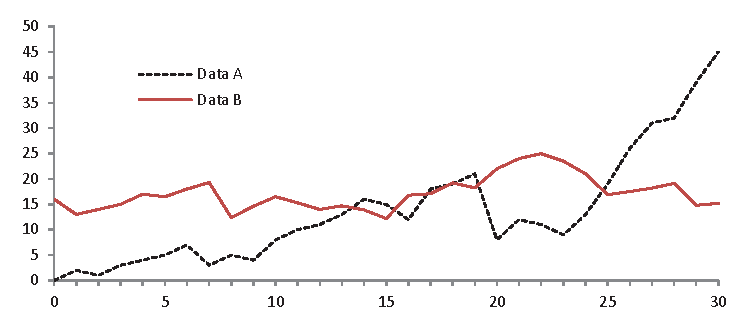
\includegraphics[width=\textwidth]{fig1.eps}
\caption{A figure caption is always placed below the illustration.
Please note that short captions are centered, while long ones are
justified by the macro package automatically.} \label{fig1}
\end{figure}

\begin{theorem}
This is a sample theorem. The run-in heading is set in bold, while
the following text appears in italics. Definitions, lemmas,
propositions, and corollaries are styled the same way.
\end{theorem}
%
% the environments 'definition', 'lemma', 'proposition', 'corollary',
% 'remark', and 'example' are defined in the LLNCS documentclass as well.
%
\begin{proof}
Proofs, examples, and remarks have the initial word in italics,
while the following text appears in normal font.
\end{proof}
For citations of references, we prefer the use of square brackets
and consecutive numbers. Citations using labels or the author/year
convention are also acceptable. The following bibliography provides
a sample reference list with entries for journal
articles~\cite{ref_article1}, an LNCS chapter~\cite{ref_lncs1}, a
book~\cite{ref_book1}, proceedings without editors~\cite{ref_proc1},
and a homepage~\cite{ref_url1}. Multiple citations are grouped
\cite{ref_article1,ref_lncs1,ref_book1},
\cite{ref_article1,ref_book1,ref_proc1,ref_url1}.
%
% ---- Bibliography ----
%
% BibTeX users should specify bibliography style 'splncs04'.
% References will then be sorted and formatted in the correct style.
%
% \bibliographystyle{splncs04}
% \bibliography{mybibliography}
%
\bibliographystyle{splncs04}
\bibliography{Ref}

\end{document}
